\subsubsection{Esquemático del circuito completo}

Se puede ver un esquemático completo de la solución en la \autoref{fig:hardware/esquematicoCompleto}. Se pueden ver los módulos con las conexiones entre ellos. En él, se pueden ver todas las conexiones explicadas previamente \todo{Ver si explico yo aqui las cosas o en el diagrama de bloques}. Está dividido en las seis zonas principales del circuito:
\begin{itemize}
    \item Entrada solar. Compuesta por el panel solar simulado y su módulo de monitorizado de tensión y corriente. Se encarga de proporcionar la tensión de entrada al circuito (cuando no se está utilizando la batería de \textit{backup}) y monitorizar sus parámetros.
    \item Batería de backup. Compuesta por el relé que conecta o desconecta la carga de la batería de backup, el cargador, el módulo de monitorización de tensión y corriente, la propia batería y el convertidor elevador. Se encarga de cargar la batería de \textit{backup}, monitorizarla y elevar su tensión para utilizarla de entrada al circuito.
    \item Selección de fuente. Módulo de relé que conmuta entre la tensión del panel y la de la batería de \textit{backup} para utilizarlas como entrada al circuito.
    \item Baterías principales. Compuesta por los dos cargadores y módulos de monitorización de las baterías a cargar.
    \item Regulador $5\ V$. Regulador reductor conmutado y regulador lineal para conseguir la tensión de alimentación para el \texttt{ESP8266} y los cuatro \texttt{INA226}.
    \item Microcontrolador. \texttt{ESP8266} encargado de tomar las medidas, almacenarlas y enviarlas y gestionar la conmutación de los relés.
\end{itemize}

\begin{figure}[H]
    \centering
    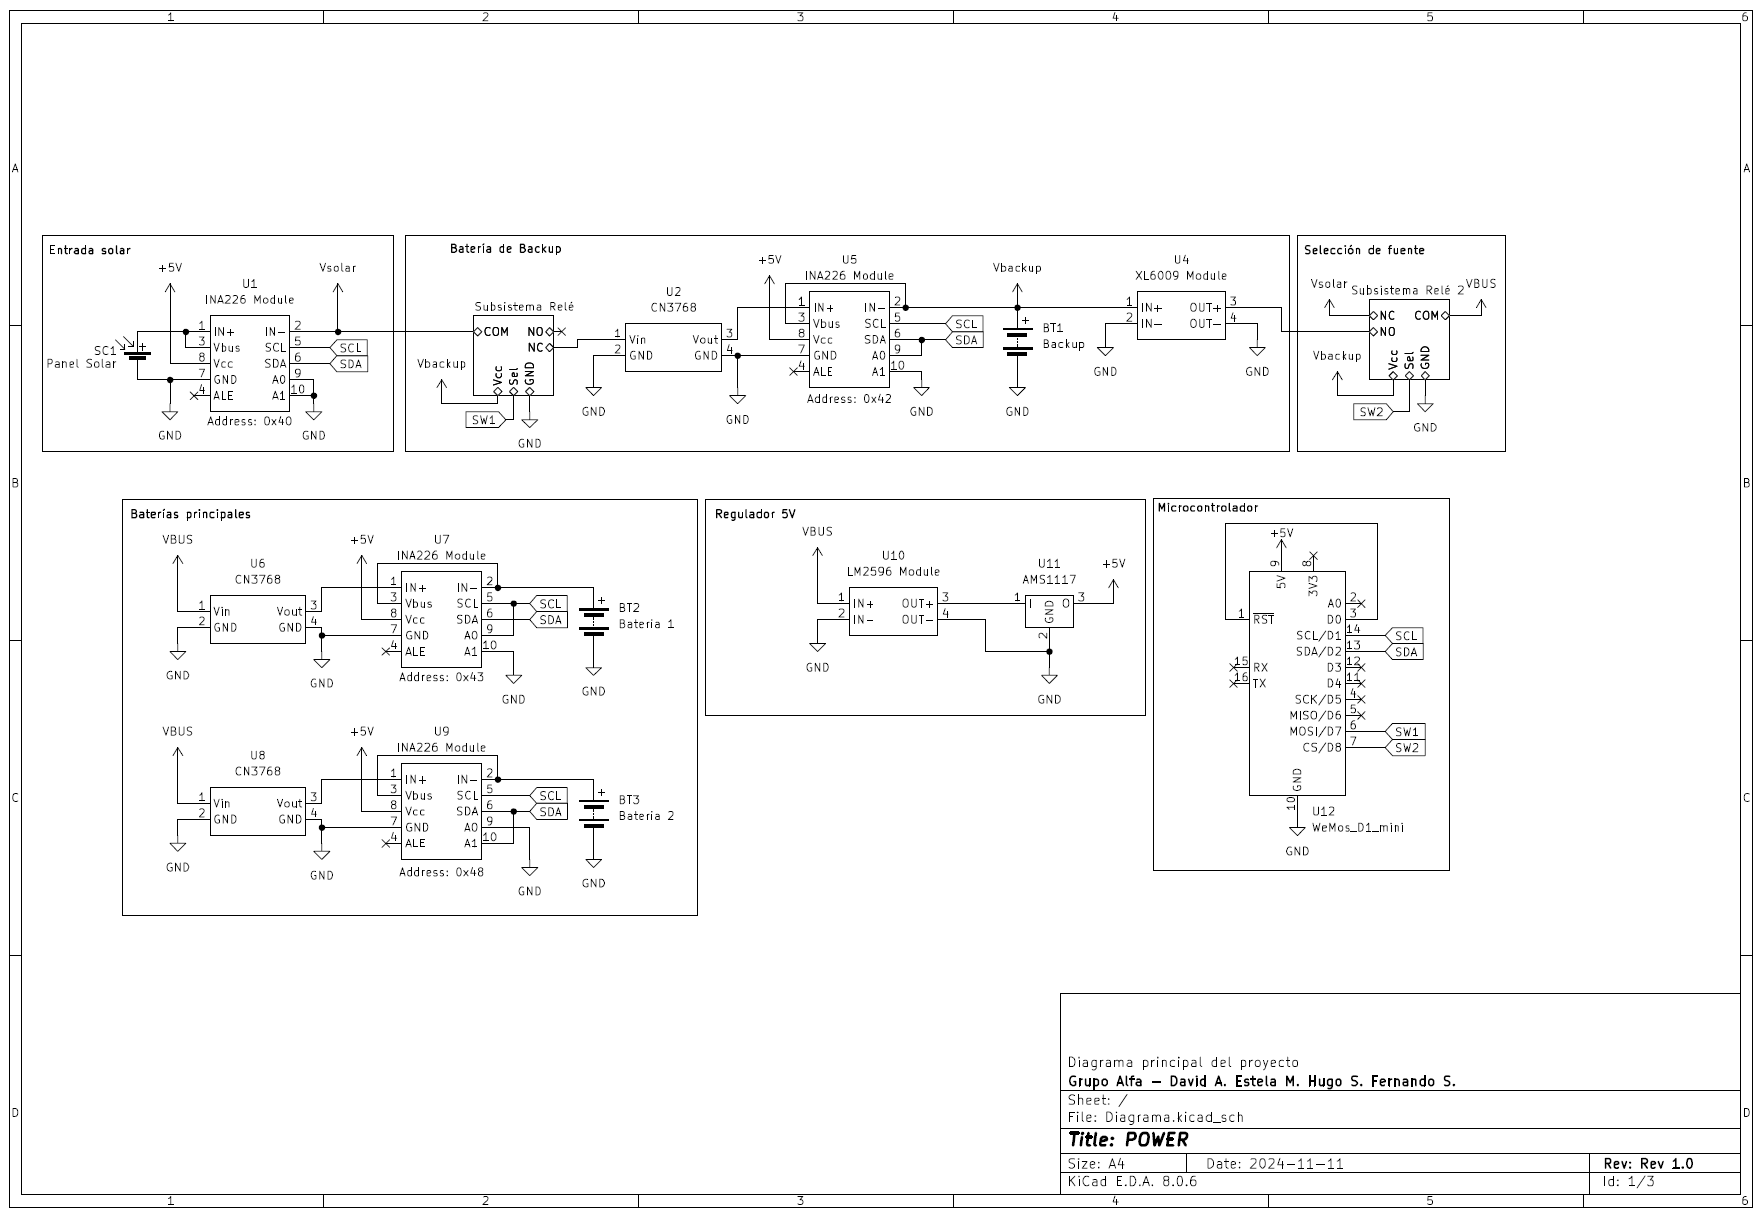
\includegraphics[width=0.95\textwidth]{images/2-hardware/esquematicoCircuito.png}
    \caption{Esquemático del circuito completo}
    \label{fig:hardware/esquematicoCompleto}
\end{figure}

En la \autoref{fig:hardware/esquematicoReles} se puede ver el esquemático preciso del circuito para los relés y el diseño de la PCB construida. La explicación de este circuito se puede ver en el \autoref{subsubsec:hardware/circuito-reles}.

\begin{figure}[H]
    \centering
    \begin{subfigure}[b]{0.65\textwidth}
        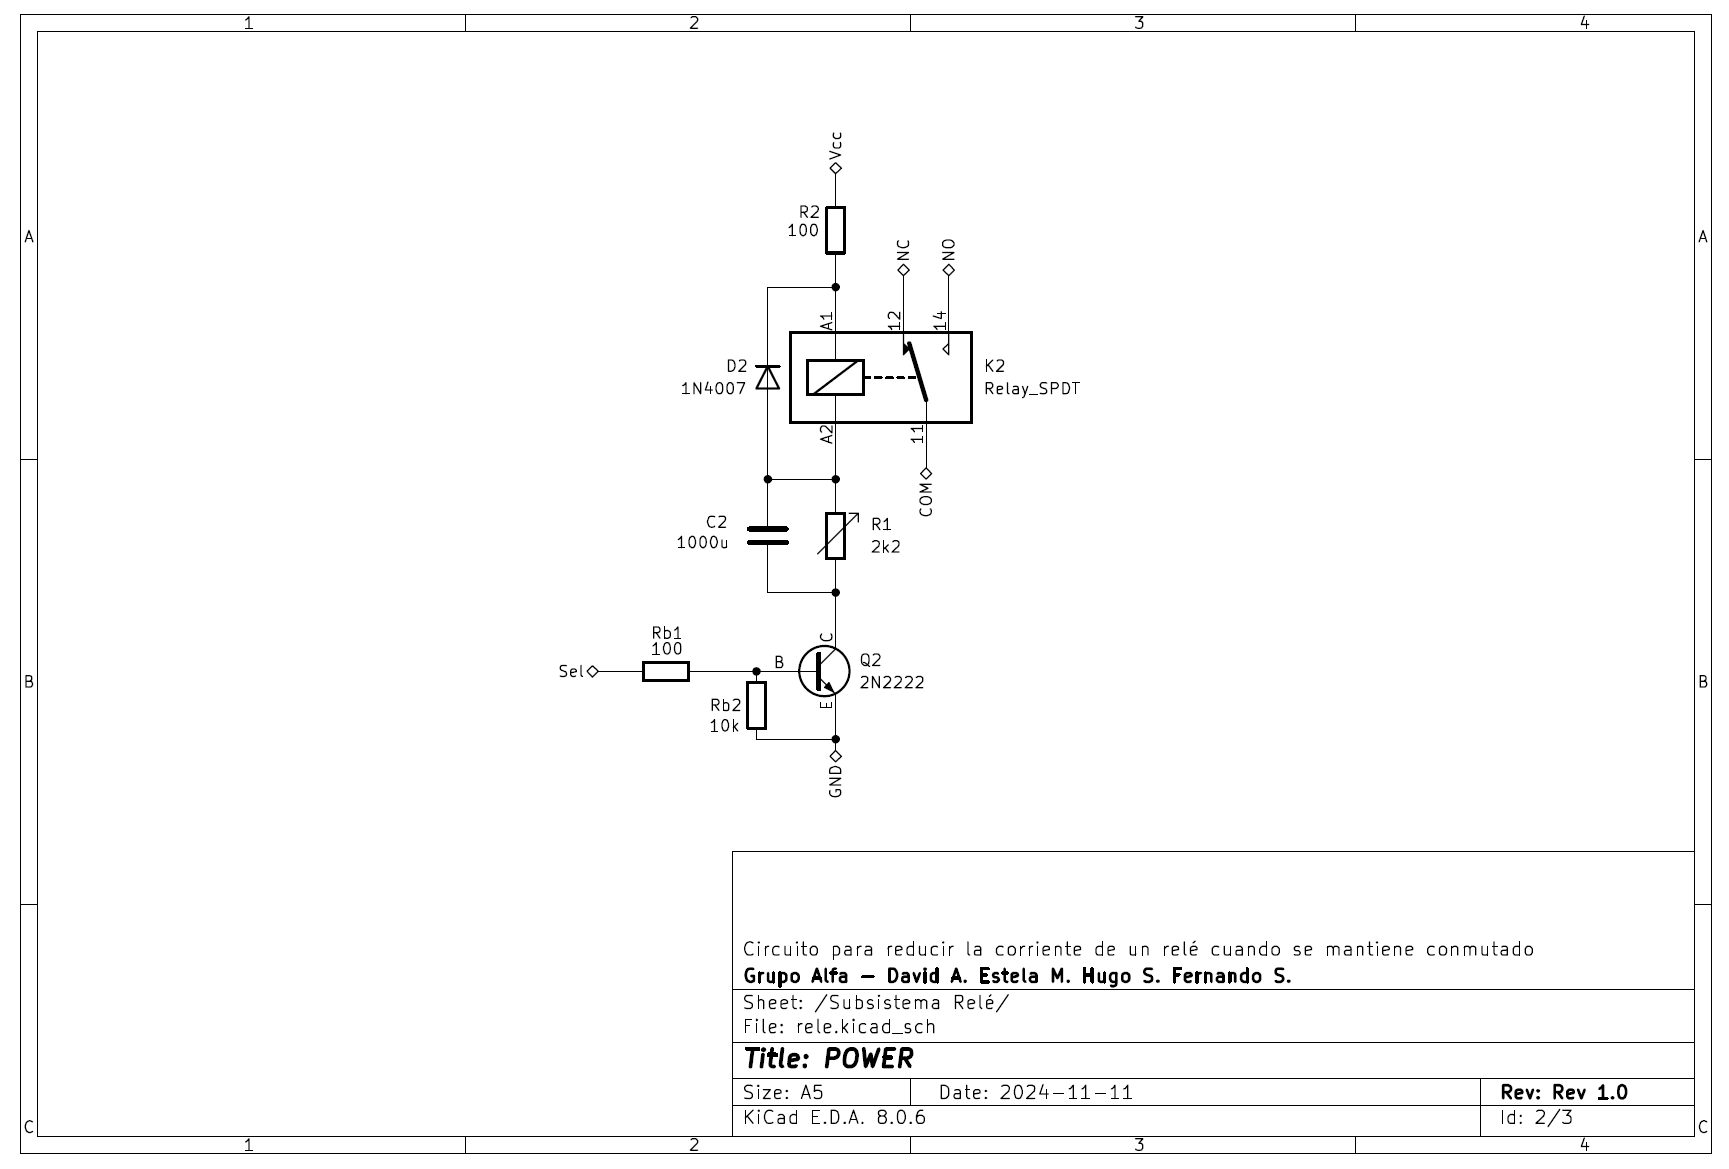
\includegraphics[width=\textwidth]{images/2-hardware/esquematicoReles.png}
        \caption{Esquemático del circuito para los relés}
    \end{subfigure}
    \hfill
    \begin{subfigure}[b]{0.3\textwidth}
        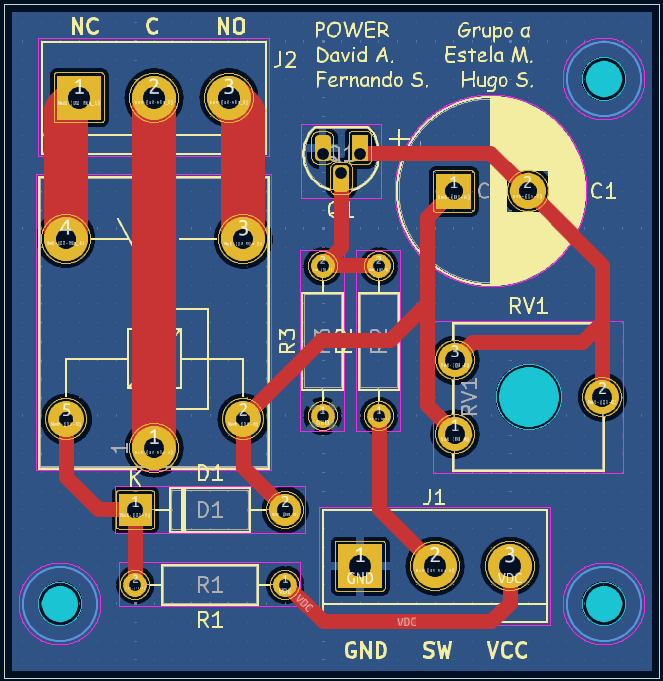
\includegraphics[width=\textwidth]{images/2-hardware/pcbReles.png}
        \caption{Circuito montado}
    \end{subfigure}
    \caption{PCB del circuito para los relés}
    \label{fig:hardware/esquematicoReles}
\end{figure}